\documentclass[10pt]{article}
\oddsidemargin -0.05in \topmargin -0.25in
\textwidth 6.5in \textheight 8.5in

\usepackage[english]{babel}
\usepackage{graphicx}
\usepackage[amssymb]{SIunits}% SI units package
\usepackage{color}
\usepackage{amsmath}
\usepackage{subcaption}
\renewcommand{\Re}{\mathrm{Re}}
\newcommand{\strong}[1]{\textbf{#1}}
\newcommand{\red}[1]{\textcolor{red}{#1}}
%\newcommand{\makered}[1]{\textbf{#1}}
\newcommand{\question}[1]{\begin{quote} \emph{#1}  \end{quote} }

\newcommand{\comm}[1]{}
\bibliographystyle{jasanum}


\begin{document}

\noindent Date: \today \\
Manuscript: IJMF\_2017\_854\\
Title: Air cavities at the inner cylinder of turbulent Taylor-Couette flow \\
Authors: Ruben A. Verschoof, Dennis Bakhuis, Pim A. Bullee, Sander G. Huisman, Chao Sun, Detlef Lohse

\vspace*{1.25cm}
\section*{Referee 1}
We thank the referee for her/his detailed reading of our manuscript, and for his/her support to publish our manuscript. We react to his/her comments below.

\question{Authors present original research on drag reduction in Taylor-Couette reactor by forming air cavities using various number of cavitators with and without air injection. Shape of the air pocket and the drag on the inner cylinder were measured and presented. Drag reduction is shown to be affected by Reynolds number, void fraction, and Buoyancy, but not the flow rate of injected air. It is shown that using a cavitator increases the total drag force compared to smooth cylinder case despite the reduction caused by the cavities. I suggest publication of this manuscript after the following revisions.}


\noindent \strong{1}

\question{Page 5 Fig 1; Void fraction measurement using water level can often be very unreliable because of the non-flat surface of the water due to rotation and change of curvature depending on the rotational speed. Please provide a sample image of the water surface and explain how measurement was done and provide the estimated uncertainty. }

\noindent \strong{Response:} 

\noindent We did not measure the void fraction instantaneously, but measured it with both cylinders at rest. As the TC setup is a closed setup --- apart from a small opening in the top to prevent pressure buildups ---, the amount of water and air inside does not change while measuring. Therefore, the void fraction must be constant while measuring. Before and after each measurement we checked the water level, to ensure a constant void fraction. The error is determined by the accuracy with which the water level can be measured, and is approximately $\alpha_{err} \leq 0.1 \%$\\
We now added more details of the void fraction measurement to our manuscript.\\
	 
\noindent \strong{2}

\question{Page 5 Fig 1; ``Turbulent mixing and the large centrifugal accelerations ensure mixing of the two phases.'' Is it important to achieve a uniform mixture for this study? 
 }

\noindent \strong{Response:} 

\noindent In our setup, we have two effects. i) turbulence mixes both phases. And ii) centrifugal accelerations separate both phases, pushing air towards the inner cylinder. It is not important to achieve a uniform mixture: we want air to be close to the inner cylinder. 
We carefully rewrote that sentence in the revised manuscript, to make our point clearer. \\

\noindent \strong{3}

\question{Page 10 Fig 6; These curves seem to suggest that at the lower Reynolds numbers, no axial dependence exists, probably due to the vertical axis not being normalized. Please clarify.}

\noindent \strong{Response:} 

\noindent At the lowest Reynolds numbers, the buoyancy forces and turbulent mixing are not yet strong enough to create a stable air layer at the three indicated heights. A small cavity is formed more towards the top: as shown in figure 7, the coverage is non-zero. \\
We now added this to the manuscript.\\

\noindent \strong{4}

\question{Page 10 Fig 7; Was integration of the cavity lengths done using only 3 axial locations of Fig 6? Was a trapezoid assumed for integration? Please explain the integration with more detail.
 }

\noindent \strong{Response:} 

\noindent We manually shade the area which was covered by a cavity, which then results in a black-white image. In here: black refers to area covered by an air cavity, the white area is not. From these images, we calculate the coverage area, and we can extract the cavity length at any height. We here chose to show 3 heights.\\
We now added more information on the photo analysis methods to the manuscript.\\

\noindent \strong{5}

\question{Page 9 Section II B; Is image distortion due to cylinder curvature accounted for in measurement of cavity length from photos? }

\noindent \strong{Response:} 

\noindent  The field of view is distorted most towards the left- and right sides of the photographs. We agree with the referee that these distortions introduce some error. To minimize the influence of curvature on the cavity length- and coverage, we only used part of the images, in which we omitted the largely distorted left- and right sides. We reconstructed the entire distance between 2 cavitators by `stitching' multiple images together. \\ 

\noindent \strong{6}

\question{Section II B; Is the void fraction maintained at 2\% and 4\% values throughout the different Reynolds numbers studied or is it assumed to not change with changing the rotation speed? }

\noindent \strong{Response:} 

\noindent The void fraction does not change with rotation speed, and thus it is maintained at the indicated void fraction. We refer the referee to our response to comment 1 for more explanation. \\

\noindent \strong{7}


\begin{figure}[htp]
\begin{center}
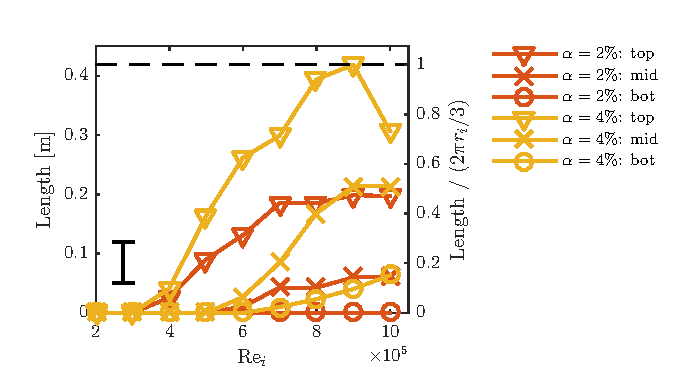
\includegraphics[scale=1.1]{fig6_new.eps}
\caption{Streamwise air cavity length on the inner cylinder as a function of $\Re_i$. }
\label{fig:length}
\end{center}
\end{figure} 

\question{Page 10 Figs 6 \& 7 and Page 12 Figs 8 \& 9; Is the same patterns of cavity length and volume seen for different number of cavitators? }

\noindent \strong{Response:} 

\noindent As is shown in fig.\ 7 of the original manuscript (shown here for the referees' convenience as fig.\ \ref{fig:length}), in almost all cases, the streamwise length is smaller than half of distance between 2 cavities. Therefore, having 2 or 3 cavitators would not change the streamwise cavity length, except for a small part close to the top of the setup at $\alpha=4\%$.  For any case that a cavity extends over multiple cavitators, the submerged cavitators do not significantly affect  the flow or the cavity, as was convincingly shown in ref.\ \cite{Zverkhovskyi2014}.\\
We now mention this in our revised manuscript.\\

\noindent \strong{8}

\question{Page 11 Section II C Paragraph 1; How much does the temperature vary during the experiments? Are the physical properties of water affected sensibly? }

\noindent \strong{Response:} 

\noindent We continuously measure the temperature, which is kept as constant as possible by active cooling of our setup. The actual temperature is kept at $(20\pm0.5) ^{\circ}C$. The density is hardly affected by these small temperature fluctuations; the change in kinematic viscosity cannot be neglected. As the temperature is measured continuously, we always calculate our dimensionless torque using the instantaneous temperature corrected water quantities. \\ In the revised manuscript we now elaborate on this in the experimental method section.  \\

\noindent \strong{9}

\question{Page 12 Fig 9; Uncertainty bars for torque measurement are needed to show that the difference in recorded value is real. }

\noindent \strong{Response:} 

\noindent We now added errors bars to all figures showing torque and DR data. \\

\noindent \strong{10}

\question{Page 17 Section III; The definition of centrifugal Froude number seems to be questionable. Gravitational acceleration is replaced with centrifugal acceleration here despite the fact that the paper shows the effect of gravity to be quite strong on the studied cavities. I would suggest providing references or explanations or maybe considering to find a more appropriate definition. }

\noindent \strong{Response:} 

\noindent We wrote this section to assist others in the field to better understand and apply our results. Basically, rather than air which is pushed upwards towards a ships' hull, we here push air radially towards the inner cylinder. The fluid experiences two body forces: i) the gravity, and ii) the centrifugal forces, both acting in different directions. Therefore, we chose to define a second Froude number, one which takes these centrifugal forces into account. \\
In our setup, we observe 2 competing effects: the buoyancy forces and the centripetal forces acting on the bubbles. Only for $\Re_i \to \infty$, we can fully neglect the buoyancy forces. For the Reynolds numbers studied in our work, both the buoyancy forces and the centrifugal forces play a role. \\
In the revised manuscript, we rewrote the accompanying text to avoid misunderstandings.\\

\noindent \strong{11}

\question{Page 17 Section III Paragraph 2; Based on the calculated Fr number, it is suggested that enough air would cover the entire cylinder even though it was previously explained that extra air would leave from the top free surface due to Buoyancy. This too might be a result of not seeing gravity in the Fr definition. }

\noindent \strong{Response:} 

\noindent We agree with the referee: if enough air would be available and with sufficiently high centrifugal accelerations, the cylinder would be completely covered by air. We stress that the global void fraction remains constant during each measurement. For more discussion on the (centrifugal) Froude number, we refer the referee to our response on comment 10.\\

\noindent \strong{12}

\question{Page 17; The paragraph after Table I does not seem to add to reader's confidence as of how valuable the results are even though the rest of the discussions show the relevance of the research. I suggest removing it, however, it is the authors? decision. }

\noindent \strong{Response:} 

\noindent We understand the point of the referee. However, we think it is crucial to highlight some of the differences between our measurements and the way air lubrication is applied in marine vessels. \\

\noindent \strong{13}

\question{It is very important for the authors to perform a careful reread of the manuscript before resubmission as there are several small grammatical errors that can be very confusing to the readers. }

\noindent \strong{Response:} 

\noindent We carefully reread the manuscript to catch the last grammatical errors and any typos.\\




	\bibliography{literatur,2ph_literatur}


\end{document}